\section{PROPOSED FRAMEWORK}
\label{sec:methods}
% overview of the framework
In this research, we propose a four-stage framework, as illustrated in Figure \ref{fig:general_framework}, that integrates methods introduced in Section \ref{sec:methods} for continuously estimating lifting risks and monitoring human ergonomics in real-time applications. A more detailed data flow of working pipelines is shown in Figure \ref{fig:pipelne_overview}.
\begin{figure}[htp]
   \centering
   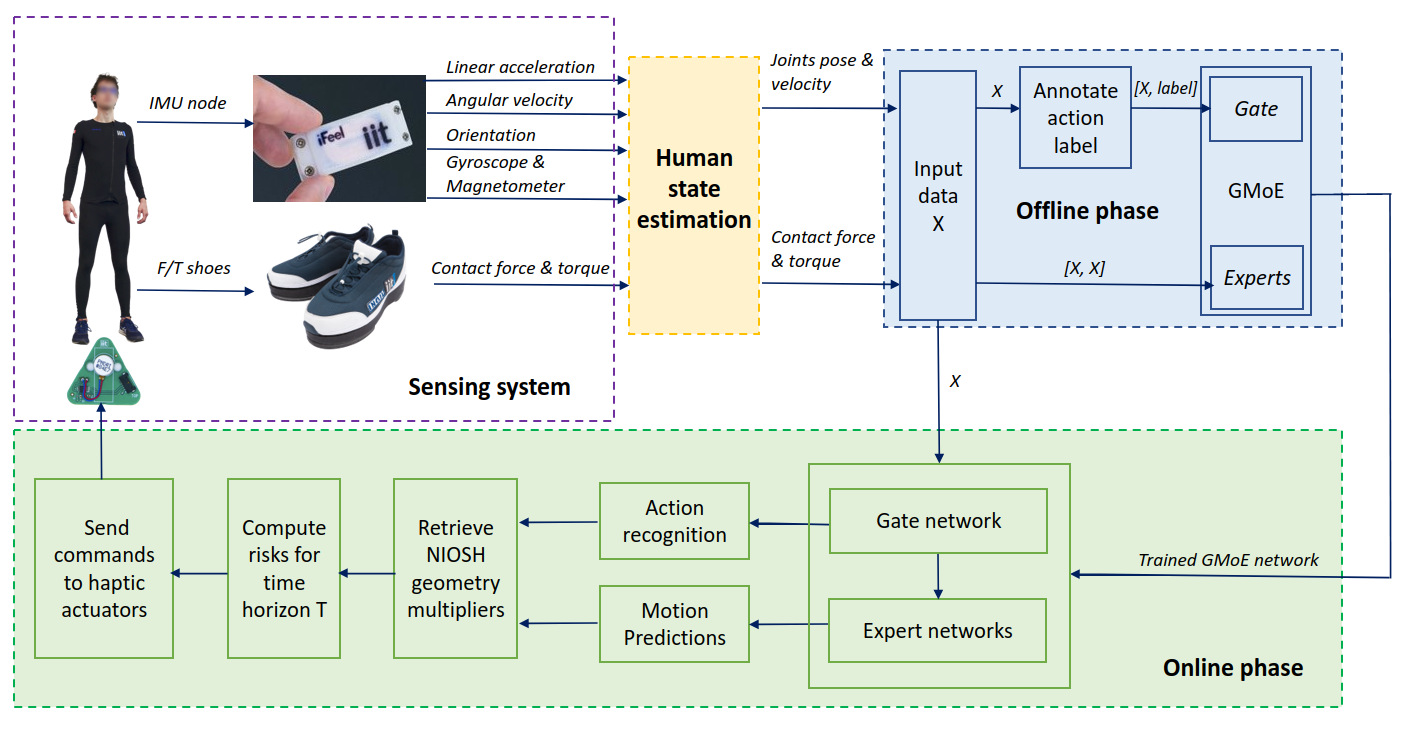
\includegraphics[scale=0.18]{figures/fig_pipeline_overview.png}
   \caption{Data flow of the proposed framework, composed of an online and offline phase.}
   \label{fig:pipelne_overview}
\end{figure}

Firstly, human kinematic measurements and ground contact force/torque are collected by \emph{iFeel node} and \emph{F/T shoes}. The sensor data are then regarded as the \emph{targets} for estimating human full-body joints/floating-base configurations (e.g. positions and velocities) and external feet wrenches (e.g. forces and torques) via Inverse Kinematics (IK) and Inverse Dynamics (ID) algorithms. Afterwards, the output of the \emph{human state estimation} module is manually annotated according to pre-defined action labels for the GMoE network training. Finally, during the online phase, combining the outputs of GMoE and IK/ID modules, the \emph{NIOSH-based method} module is able to provide risk predictions for a given time horizon and thus send commands to haptic actuators worn by human subject.

\subsection{Data Preparation}
\label{subsec:make_data}
% what is the data we collected
To apply GMoE for a lifting task scenario, we build a 15-minute dataset, with data sampled at a frequency of 100Hz. The dataset consists of two volunteers executing three types of lifting tasks repetitively, lasting for 150 seconds each. The volunteer is asked to naturally lift a 3kg payload to a certain height without twisting the upper trunk. The lifting height ranges from 68cm to 92cm, while the other variables (e.g., horizontal distance, payload weight, etc.) remain the same. 

% why we divide a single lifting activity into three phases
Assume the human subject starts with a \emph{standing} pose, a natural sequence of actions during a single lifting activity consists of \emph{squatting}, \emph{rising} and back to \emph{standing} pose again. The lifting risks are most likely to happen during \emph{squatting} and \emph{rising} phases. To apply the NIOSH equation, we must identify the starting and ending moments of each action to establish the initial and final positions of the human subject. For this purpose, we segment a single lifting activity into three continuous phases, each corresponding to a specific action, as illustrated in Figure \ref{fig:lift_activity}.
\begin{figure}[htp]
     \centering
     \begin{subfigure}[b]{0.15\textwidth}
         \centering
         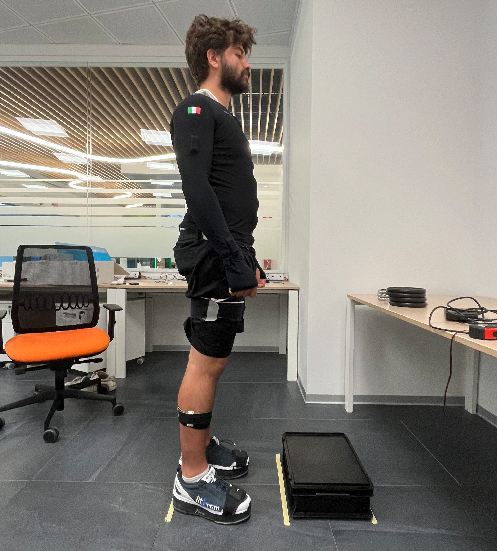
\includegraphics[width=\textwidth]{figures/gianmar_standing.png}
         \caption{\emph{standing}}
         \label{fig:lift_standing}
     \end{subfigure}
     \hfill
     \begin{subfigure}[b]{0.15\textwidth}
         \centering
         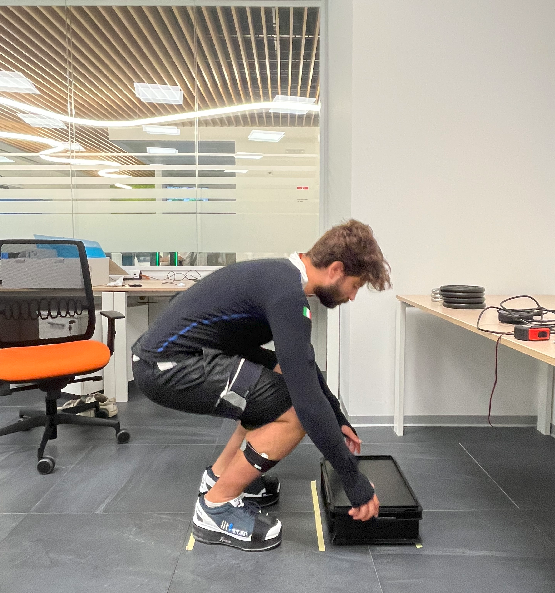
\includegraphics[width=\textwidth]{figures/gianmar_squatting.png}
         \caption{\emph{squatting}}
         \label{fig:lift_squatting}
     \end{subfigure}
     \hfill
     \begin{subfigure}[b]{0.15\textwidth}
         \centering
         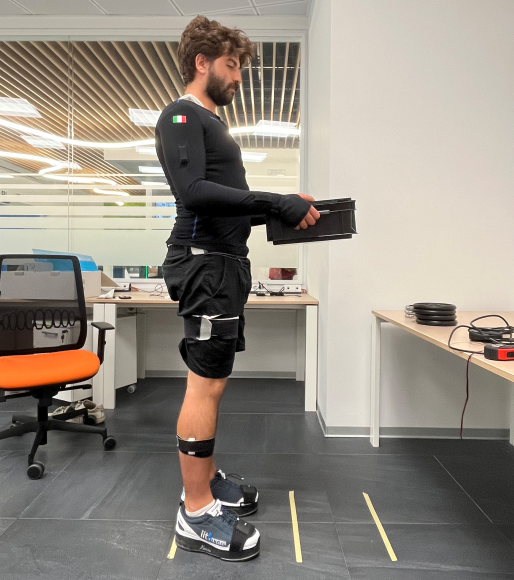
\includegraphics[width=\textwidth]{figures/gianmar_rising.png}
         \caption{\emph{rising}}
         \label{fig:lift_rising}
     \end{subfigure}
        \caption{The three phases composing the lifting activity.}
        %\LorenzoSays{[remember to change this with some new picture done in our lab]}}
        \label{fig:lift_activity}
\end{figure}

% data annotation process
Given the high cost associated with manual labeling, we have developed an autonomous tool aimed at enhancing the efficiency of annotation. In this labeling process, the estimated data for the entire human body is visualized using a URDF model, while data are streamed in a terminal with a fixed frequency. By observing the action change of the URDF model, an action label is carefully assigned to the current data frame. As long as no new label is assigned by the user, the following data frames are considered to belong to the previous action. More precisely, the transition between \emph{standing} and \emph{squatting} is discerned by observing the bending of the knee. Once the \emph{squatting} action is reaching the end, the ascent of the pelvis denote the beginning of the \emph{rising} phase. The accomplishment of \emph{rising} is detected when, observing a totally erect trunk, the label is assigned as \emph{standing} once again. In the end, the annotated data are divided into three subsets, 70$\%$ for training, 20$\%$ for validation, and the last 10$\%$ for test.

\subsection{GMoE for Lifting Activity}
% how does GMoE look like
To achieve simultaneous action recognition and motion prediction, we adopt the network model proposed in \cite{Kourosh2022}. Since three actions are considered in our case, the implemented GMoE architecture is composed of three \emph{expert} networks and one \emph{gate} network, as illustrated in Figure \ref{fig:moe_model}.

% inputs and outputs of GMoE
The input layer is of size 10x74, where 10 represents the window size for reading past data frames, while 74 is the number of input features, consisting of 31 joint positions, 31 velocities, and 12 contact forces/torques. The \emph{gate} network output layer has size 3x50, where 3 denotes the action categories, and 50 denotes the number of future frames for which action probabilities are computed. It should be noted that when generating time series data, we practically take one data frame every three time steps, such that the period between two adjacent data frames in an input sequence is 30ms. Therefore the total prediction time horizon is 1.5 seconds. Similarly, the output size of each \emph{expert} network is 3x50x43, where 31 joints' positions and 12 foot wrenches are considered (in total 43 output features), excluding the joints' velocities.

% define loss function, other ML methods used
During the training phase, the loss function $L_1$ associated with \emph{gate} network and loss function $L_2$ associated with \emph{expert} network are chosen as categorical cross-entropy loss and mean squared error loss, respectively. The total loss function L for GMoE is expressed as a linear combination of $L_1$ and $L_2$:
\begin{equation} \label{loss}
\begin{split}
L & = b_1L_1 + b_2L_2 \\
 & = -\frac{b_1}{2M}\sum_{t=1}^{T}\sum_{j=1}^{M}\sum_{i=1}^{N} a_i^{j,t}log(\tilde{a}_i^{j,t}) \\
 & + \frac{b_2}{2M}\sum_{t=1}^{T}\sum_{j=1}^{M}\|\sum_{i=1}^{N}\tilde{a}_i^{j,t}\tilde{\bm{y}}_i^{j,t}-\tilde{\bm{y}}^{j,t}\|_2
\end{split}
\end{equation}
where $b_1$ and $b_2$ are manually chosen for the convergence of both classification and regression problems (in this case, $b_1$ is 1.0 and $b_2$ is 0.5 for faster convergence of \emph{gate} network), T is the prediction time horizon, M is the total number of data frames, N is the number of experts, scalar value $a_i^{j,t}$ and vector $\tilde{\bm{y}}_i^{j,t}$ denote for human action and motion ground truth associated with \emph{i}-th action and \emph{j}-th data frame at time instance t in the future, operator $\tilde{\cdot}$ represents prediction values of both action recognition and future motions. To update the network weights, \emph{Adam} optimizer is applied with epsilon equals 1e-6. Moreover, early stopping technique and adaptive learning rate are used to avoid overfitting or local optimum. 

\begin{figure}[t]
    \centering
    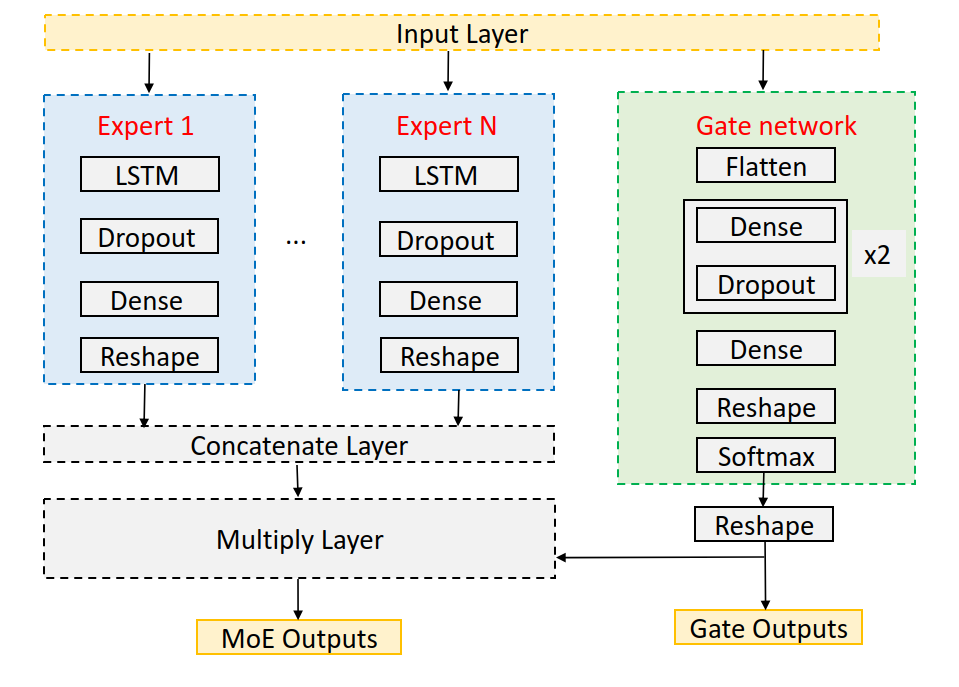
\includegraphics[scale=0.24]{figures/fig_gmoe.png}
    \caption{Adapted structure of Guided Mixture of Experts architecture for action recognition and motion prediction.}
    \label{fig:moe_model}
\end{figure}

\subsection{Risk Prediction and Haptic Alert}
\label{sec:RNLE_implementation}
% why we can realize risk estimation and prediction
% what are action recognition and motion prediction used for 
As mentioned in Section \ref{subsec:make_data}, action recognition is used to determine the origin and destination time point of each action during a single lifting activity. Once the origin status is identified, each following instant can be considered a temporary destination status, which makes it possible to use NIOSH equation to compute risk at that time. Until next action is detected, the NIOSH equation can be applied repeatedly without violating any constraints. Furthermore, by making use of predicted motions, we are also capable of predicting potential risks in the future for a given time horizon. The process of estimating and predicting risks is demonstrated in Algorithm \ref{algorithm:risk_prediction}. Once any potential risk is detected, a command will be sent to the haptic actuator mounted on the human's back. The vibration intensity of the actuator corresponds to the predicted risk level. The human can thus take appropriate measures based on the vibrotactile feedback, i.e., to abort the task immediately or adjust only the lifting posture.
\begin{algorithm}[b]
\caption{Risk prediction using RNLE}
\label{algorithm:risk_prediction}
\begin{algorithmic}
\Require action at $t_0$: $A_{t_0}$, action at $t$: $A_t$, motion prediction at $t$ for future N steps: $M_{t}^{t+N}$, human origin status at $t_0$: $S_{t_0}$, NIOSH variables: $A$, $C$, $F$
\Ensure risk prediction at $t$ for future N steps: $R_t^{t+N}$
\State Initialize $R_t^{t+N}$
\While{$True$}
\If{$A_t$ is not $A_{t_0}$} \Comment{Detect next action}
    \State $A_{t_0} \gets A_t$
    \State $S_{t_0} \gets getHumanStatus(M_{t}^{t+N}[0])$
\EndIf
\For{each item $i$ in $M_t^{t+N}$}
    \State $S_t \gets getHumanStatus(M_{t}^{t+N}[i]))$ 
    \State $H, V, D \gets getVariables(S_{t_0}, S_t)$
    \State $R_t^{t+N}.append(RNLE(H,V,D,A,C,F))$
\EndFor
\State return $R_t^{t+N}$
\EndWhile
\end{algorithmic}
\end{algorithm}

% compensation method to detect action change
In practice, the action transition cost about 0.5s, which affects the accuracy of action detection. To retrieve more precise NIOSH variables, we implement an approach to compensate action change delay. At each moment, when the probability of previously recognized action is growing, the current action label maintains the same. Once the probability decreases over a pre-defined threshold, we consider the action transition already starts. Then we search for the action label whose probability increases also over a threshold. 

% NIOSH variables retrievement
As shown in Algorithm \ref{algorithm:risk_prediction}, from predicted motions we can update the human model in simulator and retrieve geometry values to compute NIOSH variables \emph{H}, \emph{V} and \emph{D}. Assume that the middle point of human hands is always overlapped with the Center of Mass (CoM) of the payload, \emph{H} can be thus represented as the horizontal distance between the position of the CoM of human hand w.r.t. the frame attached to human foot, while \emph{V} is computed by using the vertical position of the human hand w.r.t. the human foot:
\begin{subequations}
\begin{align} \label{eqa_H}
& H = \frac{H_{LeftHand}^{LeftFoot} + H_{RightHand}^{RightFoot}}{2} ~,\\
\label{eqa_V}
& V = \frac{V_{LeftHand}^{LeftFoot} + V_{RightHand}^{RightFoot}}{2} ~.
\end{align}
\end{subequations}
and vertical traveling distance is denoted as \(D = V_t - V_{t_0}\),  where $V_t$  and $V_{t_0}$ represent the vertical distance at the destination and origin moment, respectively. For simplification, asymmetry angle $A$ is not considered in our case, hence $AM$ constantly equals 1. Lifting frequency is computed as the average number of lifts per minute over a 15-minute period. The coupling situation is considered as \emph{Fair}.

% mention the haptic alert here


